\chapter{Foundations}\label{foundations}
Most of the groundwork of the methods we will be using was invented in the second half of the 20th century. They include reinforcement learning---a general framework defining the aim of the playing algorithm, Q-learning---a simple algorithm to learn to play a game, and basics of neural networks---the statistical model that was used to overcome Q-learning's limitations.
This foundation work, joined with the recent (after $2010$) advances in the methods of training and architectures of neural networks allowed to vastly improve the former results.

This chapter discusses these methods, as well as describes the Atari machine, as the games we are interested in playing are created for this platform.

\section{Reinforcement learning}
To create an algorithm learning to play a game or solve any other problem, we first have to formally define what the problem is. We will model Atari games within the framework called reinforcement learning. The main property distinguising reinforcement learning problems from supervised learning (prediction) and unsupervised learning (clustering) is presence of two separate entities: the \emph{environment} and the \emph{agent}.

The environment is the physics or the rules of the game. It presents state, which can be any description of the game, to the agent, scores its action and provides him with the following state.
The agent is the algorithm we prepare. It receives a state it is in from the environment, decides which action to choose there and receives the appropriate reward. Every move happens in a discrete moments of time.

The aim of the creator of the reinforcement learning algorithm is to invent a way to map the game state for each time $t$: $s_t$ to the action $a_t$ (possibly storing some inner state), so that the sum:
\begin{equation} \label{discounted-reward}
\sum_{k=0}^{\infty} \gamma^k r_{t + k}
\end{equation}
is maximized. $r_T$ is the reward received after doing action $a_T$ in state $s_T$ The exponential averaging is called a \emph{discounted} sum, and $0 < \gamma \le 1$ is called a \emph{discount factor} corresponds to the level of comfort we have with receiving the awards not now, but in the future. This resembles the way people evaluate their gains---if one is promissed a constant amount of money, he'd prefer to receive it rather earlier than later. We assume that every game eventually will find itself in a \emph{terminal} state, which always transistions to a terminal state and gives reward $0$. One such progression from the start of the game to reaching a terminal state is called an \emph{episode}.

Both agent and environment are not bound to make their decisions deterministically---in fact, it may be favorable for the agent to play randomly to some extent. In the stochastic case, the aim of the agent is to maximize the discounted sum of expected value of the rewards.

\begin{figure}[!h]
  \center
  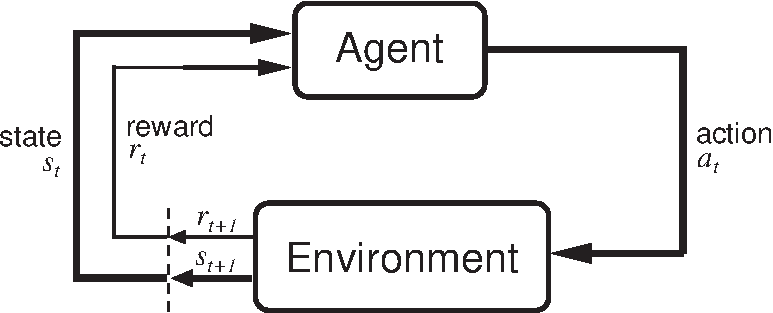
\includegraphics[scale=0.8]{images/Agent-Env-crop.pdf}
  \caption{The interaction between the agent and the environment, from \cite{reinforcement-book}.}
\end{figure}

The reinforcement learning, as defined above is a very general framework which can describe a broad range of problems. To make it easier to model it using statistical tools, we assume all the problems we consider are of the form of Markov Decision Process.

Markov Decision Process (MDP) is a reinforcement learning problem where a distribution of the following states $s_{t+1}$ and the rewards $r_t$ depends only on the previous state $s_t$ and the action $a_t$ (we assume reward $r_t$ is rewarded after choosing action $a_t$):
\begin{equation} \label{mdp}
  p(s_{t+1}, r_t|s_t, a_t, s_{t-1}, a_{t-1}, \ldots, s_0, a_0) = p(s_{t+1}, r_t|s_t, a_t)
\end{equation}

This simplifying assumtion can be summarized as "agent has all the information he needs for making actions encoded in the state". One should note that the representation of the state and not the inner mechanics of environment, is crucial here---imagine a chess-playing player, which sees only bottom half of the board. Even though the game is completely deterministic (assuming deterministic strategy of agent and environment, choosing oppontents' moves), agent cannot reliably predict what will be the next state, as there may be pieces on the other part of the board he cannot see yet.

In the case of Atari games played based on the RAM state, the MDP assumptions are satisfied. The code of the game (saved on ROM), together with a random seed for the game define a deterministic function transforming the RAM (the game state) and awarding rewards.

It is worth noting that the algorithms based on markovian assumption (TD-learning, Q-learning, Markov Chain Monte Carlo) are often used dispite the violation of assumption by the environment. The intuition behind that when the state contains enough information for agent to reasonably approximate the next state and reward distribution, it doesn't matter the approximation will not be accurate. One example of this fact is when we train agents to play Atari games based on the screen state \cite{nips-dqn}---the player moves influence the inner state (RAM) of the machine, but the changes may not be immediately apparent on the screen. Still, the game screen gives a lot of information about the game state needed to make an action, thus 
agent can fairly skillfully learn to make good decisions.

\section{Q-learning}
Let's call the function (distribution) mapping the current state $s$ to the action $a$ choosen by the agent \emph{a strategy} (or \emph{policy}) $\pi$.

An algorithm able to choose a strategy in an MDP we will discuss is called Q-learning \cite{qlearning, qlearning-old}. It is based on the notion of Q-value: a function mapping the state-action pair $(s, a)$, for a fixed strategy $\pi$ to the expected discounted reward after being in the state $s$, making an action $a$ and following the strategy $\pi$ until the end of the episode.
\begin{equation}\label{q-value}
  Q^\pi(s_t, a_t) = \underset{r\sim p(r_t | s_t, a_t)}{\mathbb{E}} r + \sum_{k=t+1}^\infty \gamma^{k-t}\underset{r\sim p(r_k|s_{k-1}, a_{k-1}), a_k\sim \pi(s_k)}{\mathbb{E}} r
\end{equation}
where $s_k$ is a random variable describing distribution of the state in time $k$, dependent of the previous state and action, as in equation \eqref{mdp}. From here on, though, we will assume that choice of the next states and rewards by the envirnoment as well as of actions by the agent are done deterministically---it will simplify the notation and all the statements will hold for the stochastic case when wrapped with the expectation signs.

The Q-learning algorithm makes use of the following property:
The strategy $\pi$ is optimal (maximizes the expected discounted reward) if and only if
\begin{equation}\label{qlearning-property}
  Q^\pi(s_t, a_t) = r_t + \gamma \max_a Q(s_{t+1}, a)
\end{equation}
for all state-action pairs.
\todo[noinline]{Maybe prove that fact: left -- for optimal strategy we can do greedy actions, right -- assume strategy is not optimal but property satisfied, then there's a better strategy that does different action somewhere, but this action leads to lower Q}

Q-learning is a representative of a general domain of algorithms called Generalized Policy Iteration (see Chapter 4.6. in \cite{reinforcement-book}). Their approach is to take turns between updating the estimation of the value of the states (in our case Q-values) and updating the strategy to take into account new state value estimation.
 
In case of Q-learning, the chosen strategy is a greedy one, i.e. it always chooses the action maximizing the immediate reward plus discounted value of the following state:
\begin{equation}
  \pi(s_t) = \argmax_a \big(r(s_t, a) + \max_{a^*} Q^\pi(s_{t+1}, a^*)\big)
\end{equation}
where $r(s, a)$ is the immediate reward after making action $a$ in state $s$ and $s_{t+1}$ is a (convenient notation for a) next state after making action $a$ in state $s_t$.

The update to the Q-values is being made to force more state-action pairs to satisfy property \eqref{qlearning-property}:
\begin{equation}
  Q_{new}(s_t, a) := \alpha Q_{old}(s_t, a) + (1 - \alpha)\big(r(s_t, a) + \max_{a^*} Q_{old}(s_{t+1}, a^*)\big)
\end{equation}
$\alpha$ (also called step-size) is a parameter of the algorithm deciding how fast should it move the q-value estimations toward the ones locally satisfying \eqref{qlearning-property}. Bigger values lead to faster training, but the convergence proof for constant step-size requires sufficiently small $\alpha$ \cite[section~3.]{qlearning-old}. It was also shown in \cite{qlearning-convergence}, that the Q-learning algorithm converges when the variable step-size satisfies:
\begin{equation}
  \sum_i \alpha_i = \infty, \;\;\;\; \sum_i \alpha_i^2 < \infty
\end{equation}

Assuming we store all the state transitions as $next\_state[s, a]$ and the rewards as $reward[s, a]$\footnote{in the non-deterministic case these can be approximated by, respectively, observed distribution of the next states and the sample average of rewards in each state-action pair}, the Q-learning algorithm can be written as:

\begin{algorithm} \label{qlearning-pseudo}
  \For{all state-action pairs$ (s, a)$}{
    $Q[s, a] = 0$ \tcp{ initialize Q-values of all state-action pairs}
  }
  \For{all states $s$}{
    $P[s] = random\_action()$ \tcp{ initialize strategy}
  }
  \While{not converged}{
    \For{all states $s$}{
      $P[s] = \argmax_a (R[s, a] + \gamma \max_b(Q[next\_state[s, a], b]))$
    }
    \For{all state-action pairs$ (s, a)$}{
      $Q[s, a] = \alpha(R[s, a] + \gamma \max_b Q[next\_state[s, a], b]) + (1 - \alpha)Q[s, a]$
    }
  }
  \caption{Pseudocode of Q-learning.}
\end{algorithm}
\section{Neural networks}
Many of the current advances in various domains of AI are the effect of improvements of an old\footnote{The predecessor of today's neural network, perceptron, was invented in $1958$ \cite{perceptron}.} statistical model, inspired by how the brain works: neural network. In this section we define it formally and describe the process of finding best parameters for it.

\subsection{Feedforward neural network}
The simplest neural network, called \emph{feedforward} neural network or \emph{multilayer perceptron} was introduced in 60's \cite{mlp}.
It consists of a couple of \emph{layers}:\footnote{In current state-of-the-art models, the number of layers reaches thousands, see e.g. \cite{stochastic}} each layer accepts some inputs, processes them, and outputs them as an input for the next layer (see figure \ref{ann-layers}). The first layer is called input layer, the last---ouput layer and all the layers in between---hidden layers.
\begin{figure}[h]   \centering
  \resizebox{0.6\textwidth}{!}{
  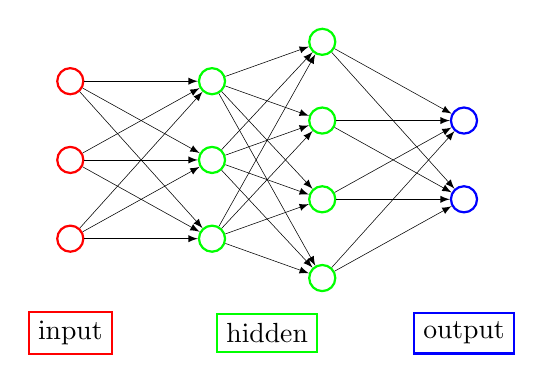
\begin{tikzpicture}

\begin{scope}[very thin]
\foreach \x in {0, ..., 2} {
\node[circle, draw, color=red, thick] (input \x) at (-3, \x) {};
}
\foreach \x in {0, ..., 2} {
  \node[circle, draw, color=green, thick] (hidden1 \x) at (-1.2, \x) {};
  \foreach \y in {0,...,2}
    \draw[-latex] (input \y) -- (hidden1 \x);
}

\foreach \x in {0, ..., 3} {
  \node[circle, draw,color=green, thick] (hidden2 \x) at (0.2, \x-0.5) {};
  \foreach \y in {0, ..., 2}
    \draw[-latex] (hidden1 \y) -- (hidden2 \x);
}

\foreach \x in {0, ..., 1} {
  \node[circle, draw,color=blue, thick] (output \x) at (2, \x +0.5) {};
  \foreach \y in {0, ..., 3}
    \draw[-latex] (hidden2 \y) -- (output \x);
}

\node[rectangle, draw, color=red, text=black, thick] () at (-3, -1.2) {input};
\node[rectangle, draw, color=green, text=black, thick] () at (-.5, -1.2) {hidden};
\node[rectangle, draw, color=blue, text=black, thick]() at (2, -1.2) {output};
\end{scope}
\end{tikzpicture}

  }
  \caption{Architecture of nodes in a feedforward neural network. Each node receives the outputs of the previous layer.}\label{ann-layers} 
\end{figure}

A layer is a composed of \emph{nodes} (also called \emph{neurons}). A node accepts as input the previous layer's nodes' outputs, calculates a linear combination of them and applies a nonlinear function, called \emph{activation} function to the result (see \ref{ann-nodes}). The typical choices for the activation function are sigmoid: $\frac{1}{1 + e^{-x}}$, hyperbolic tangent, and (popularized recently) rectified linear unit: $\max(0, x)$. 
\begin{figure}[h]
  \centering
  \resizebox{0.7\textwidth}{!}{
  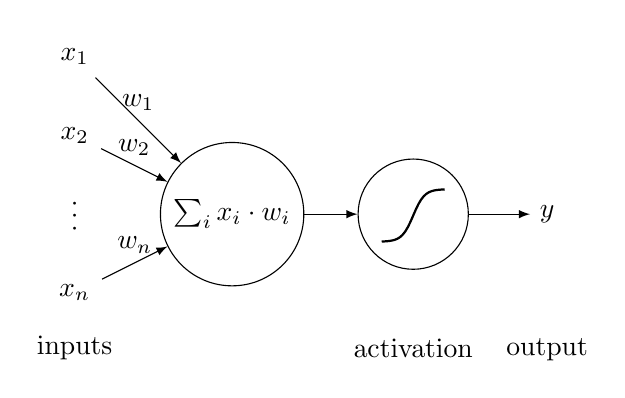
\begin{tikzpicture}[]
\node[circle](x1) at (-2, 2) {$x_1$};
\node[circle](x2) at (-2, 1) {$x_2$};

\node[circle](xn) at (-2, -1) {$x_n$};
\path (x2) -- node[rotate=90]{\ldots} (xn) ;
\node[circle, draw](center) at (0, 0) {$\sum_i x_i \cdot w_i$};
\node[circle, draw, minimum width=1.4cm](activ) at (2.3, 0) {};
\node (output) at (4, 0) {$y$};

\draw[domain=1.9:2.7, thick] plot (\x, {1/(1.5*(1+exp(-14*(\x-2.3)))) - .35});

%\draw[thick] (1.85 , -0.2) --  (2.5, -0.2) -- (2.8, 0.4);

\draw[-latex]  (center) -- (activ);
\draw[-latex] (x1) -- node[above]{$w_1$} (center);
\draw[-latex] (x2) -- node[above]{$w_2$}(center);
\draw[-latex] (xn) -- node[above]{$w_n$}(center);
\draw[-latex] (activ) -- (output);

\node ( ) at (-2,-1.7) {inputs};
\node ( ) at (2.3,-1.7) {activation};
\node ( ) at (4,-1.72) {output};

\end{tikzpicture}

}
  \caption{Details of a neural network node.} \label{ann-nodes}
\end{figure}

The trainable parameters of the model are weights of the linear combination of each of the nodes. The intuition behind introducing multilayer, multinode architecture is that different nodes will learn different statistics useful for producing the output, e.g. eye or nose detectors for face recognition. The neurons from the earlier layers will learn simple dependencies in the data (e.g. detection of edges) and the further neurons will combine their information, finding more sophisticated relations (e.g. dog detector neurons).

\subsection{Gradient descent}
There are a lot of optimization algorithms used to train neural networks, i.e. find the best set of parameters (weights) for a given network architecture and the data. All of them are a modification of a simple algorithm of gradient descent.

To use it, we first need to choose a loss function, which is a differentiable function of the output of the neural network that correlates with how well the model is doing its job; its value should be high for the bad models and low for the good  models. For example, if we want to predict the depth of each pixel in a photo (useful e.g. for self-driving cars), we could use a dataset of images acompanied with their depths estimated with a 3D camera. As a loss function, we could use a mean-squared error between the real depths and those predicted by the model:
$$
L = \frac{1}{\mbox{\# images}}\sum_{image} \sum_{x, y} (\mbox{real\_depth}(image, x, y) - \mbox{model\_output}(image, x, y))^2
$$

Then, to update the weights of the model to minimize the loss, gradient descent calculates the gradient of the loss with respect to every parameter of the model and moves the weights in the direction of the steepest descent by a small amount $\varepsilon$, called \emph{step size} or \emph{learning rate}. Choice of a bigger $\varepsilon$ leads to faster learning, but makes the optimization prone to missing good areas of space or diverging completely. Smaller step size leads to more stable
learning.

The gradients of every weight is determined with the help of chain rule:
\begin{equation}\label{chain rule}
  \frac{d}{dx} (f \circ g) = (\frac{d}{dx} f \circ g\big) \cdot \frac{d}{dx}g
\end{equation}
The equation \eqref{chain rule} suggests an order in calculating the derivatives: we should first calculate the ones of the weights in the output layer, then previous hidden layer, and so on until the input layer. For example with squared error, sigmoid activation function, datapoints $x_i$, and target outputs $y_i$ we have:
\begin{multline}
  \frac{\partial L}{\partial w_{\text{input}, 1}} = \frac{\partial}{\partial w_{\text{input}, 1}} \sum_{i} (y_i - \text{output}(x_i))^2 =\\=  \sum_{i} 2(y_i - \text{output}(x_i)) * \frac{\partial}{\partial w_{\text{input}, 1}}
  ( y_i - \text{sigmoid}(\sum_j w_{\text{output}, j} \cdot \text{hidden}(x_i, j))) =\\=
  \underbrace{\sum_{i} -2(y_i - \text{output}(x_i)) * \text{sigmoid'}(\sum_j w_{\text{output}, j} \cdot \text{hidden}(x_i, j)) * \sum_j \text{hidden}(x_i, j)}_{\sum_j \frac{\partial L}{\partial w_{\text{output}, j}}} * \frac{\partial}{\partial w_{\text{input}, 1}}\ldots
\end{multline}

Because the process of gradient calculation proceeds from the end of the network toward the beginning, it is called \emph{backpropagion} or \emph{backward pass} (in contract to \emph{forward} pass, when the network is evaluating outputs).

The calculation of a full loss, based on all examples can be infeasible: current datasets often consist of tens of gigabytes of data (see e.g. coco challenge dataset: \cite{coco-dataset}) and to train a network it is often needed to make a couple of thousands of parameter updates.
To speed the process up, it is common to approximate the full loss function (thus the gradients, too) by a loss calculated on a random subset of data examples. More often than not, a random subset of a $100$ examples will possess statistical properties indistinguishable from the whole dataset, leading to accurate (and fast to obtain) estimates of gradients. This process is called \emph{minibatch} training (and the whole algorithm a \emph{stochastic} gradient descent) and the size of the \emph{batch} is another hyperparameter of the model. There is a tradeoff in its choice---bigger batch size gives better gradient estimates, but takes longer to calculate.

The role of nodes in a neural network is symmetric---there's no reason a particular neuron should behave differently than its neighbor. To enforce neurons to learn various aspects of the data, we initialize the weights randomly. The experiments show that it suffices to make different neurons learn different weights---intuitively, the model with different neurons will have easier time predicting output, as it will be combining various types of information.

One can summarize this section in a stochastic gradient descent pseudocode:
\begin{algorithm} \label{sgd-pseudo}
  initialize all weights randomly\;
  \While{\text{not converged \& not exceeded maximum number of iterations}} {
    pick a random subset $S$ of data examples\;
    calculate the loss function for the examples in $S$ in forward pass\;
    calculate the gradients of the loss and update each weight in a backward pass:
    $w := w - \varepsilon \cdot \frac{\partial L}{\partial w}$
  }
  \caption{Pseudocode of gradient descent.}
\end{algorithm}

\section{Deep Learning}
The neural networks were not often applied in modelling until recently. There was a number of factors which contributed to their current successes. In this section we describe shortly the most important of them.

\subsection{Computing power}
Creating top prediction or classification models requires a lot of computation power.\footnote{Deep learning community jokes that the time to train a state-of-the-art model stays a week, regardless of the rapid increase in the computing power.} Neural networks, with their big expression power can provide good results, but only when supplied with enough data. When we pass a little data to a deep neural network, we can often see an \emph{overfitting} effect---the model performs well on the data it saw (training data), but generalizes poorly to unseen examples (test data). 

In a world with limited computation power, best results will be biased towards simpler models, like linear regression, random forest, or support vector machines. Out of the whole continuum of $R^n \rightarrow R^m$ functions, elementary models will pick a small subset of smooth, easy, reasonable ones and will pick the best one with the use of limitted data. As the subset of functions that can be expressed is small, they are quite different and the best model would be picked.

When a more involved model is trained, it can represent more function, but at the expense that it requires more data (thus more computation power). When faced with data scarsity, it doesn't choose the best function among all that it can represent---it falsely detects noise in the data as significant patterns and erroneusly treats insufficiently often occuring patterns as noise.

Fotunately, thanks to game industry, we saw a rapid increase in computation speed and memory bandwidth of graphics processing units (see figure \ref{nvidia-speed}). These processors allow for executing matrix operations much faster than regular CPUs. Both forward and backward passes of a neural network can be expressed as a few matrix operation, leading to efficient training of neural networks on GPU. In out experiments we saw more than ten-fold speedups moving from a high-end CPU to a middle range GPU.

\begin{figure}[h]
  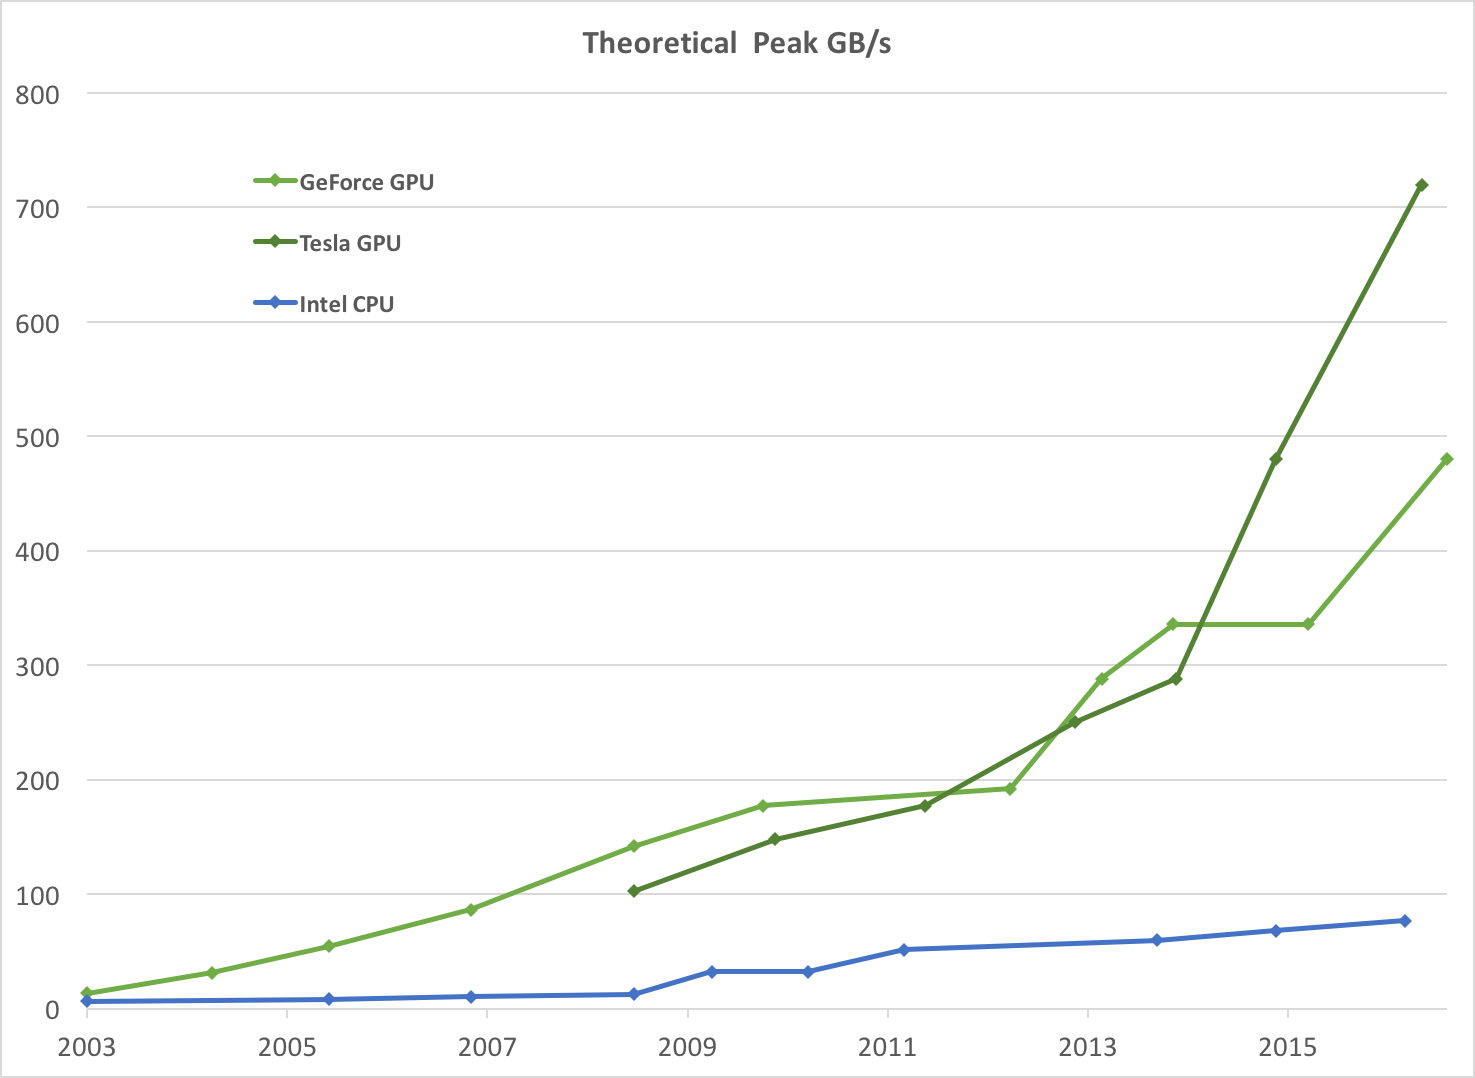
\includegraphics[width=\linewidth]{images/gpu-bandwidth.png}
  \caption{Comparison of best CPU and GPU memory bandwidths in time. Note that the memory bandwidth often constraints the speed of neural network training. Plot comes from \cite{nvidia-docs}}\label{nvidia-speed}.
\end{figure}
\subsection{Vanishing and exploding gradients}

\todo{relu saturation}

\subsection{Better training algorithms}

\subsection{Convenient libraries}

\todo{Tell that there came much faster GPUs, which allowed to have deeper networks evaluated quickly}
\todo{Tell that there were invented algorithms that better move in the multidimensional space of parameters, faster converging to a better local minimum}
\todo{Tell that it was not expected and cite Krizhevsky paper}

\todo{Tell about libraries: Torch, Theano, Tensorflow, the latter two allow for automatic differentiation}
\todo{Tell about libraries built on top of these: Keras, blocks, TFLearn}

\section{Atari 2600}
\todo{Tell about the "architecture" of the Atari machine}
\todo{Tell about the different games}
\todo{Tell about creation of ALE}
\todo{Tell about creation of OpenAI}
